\documentclass[11pt,colorlinks=true,a4paper]{article}
\usepackage[pdfauthor={Charlotte Thomas},pdfcreator={LaTeX},pdfsubject={Rapport TIPE},pdftitle={Approche pratique de la théorie des langages formels},pdfkeywords={OCaml,formal languages,pastries}]{hyperref}
\usepackage[french]{babel}
\usepackage[a4paper]{geometry}
\usepackage{float}
\usepackage{caption}
\usepackage[utf8]{inputenc}
\usepackage[T1]{fontenc}
\usepackage{listings}
\usepackage{graphicx}

\newcommand{\bsf}{Baguette\# }
\newcommand{\bs}{B\# }
\title{Approche pratique de la théorie des langages formels. \\ Rapport de TIPE}
\author{Charlotte THOMAS}

\begin{document}
    \maketitle
    \begin{abstract}
        L'informatique théorique et principalement dans l'analyse théorique des langages formels m'a toujours intéressé, 
        l'idée de créer un langage et d'en implémenter moi-même sa grammaire, son lexer,parser, interpreter et en 
        calculer les propriétés théoriques m'a vraiment intéressée et motivée.

        Les erreurs de compilation peuvent coûter cher, et parfois se compter en vies humaines, il est donc 
        nécessaire de développer des outils et des théories dans le domaine de la théorie des langages formels 
        pour prévenir les bugs en amont, et protéger des vies et la société.

        Pour illustrer ceci ce rapport va parler de la création du \textit{\bsf} (à prononcer "Baguette Sharp") un langage 
        de programmation exotique avec une syntaxe proche d'un BASIC, basé sur des pâtisseries.
        Le REPL est disponible sur OPAM \textit{opam install baguette-sharp}, le code source est sur \href{https://github.com/coco33920/ocaml-baguettesharp-interpreter}{GitHub}
        sous licence MIT, enfin le site web est disponible à cette adresse \url{https://www.baguettesharp.fr}

        Finalement, ce rapport traitera essentiellement de l'implémentation d'une Binary Turing Machine en \bs pour plus 
        de renseignements généraux merci de voir les liens au ci-dessus.
    \end{abstract}
    \tableofcontents
    \listoffigures
    \cleardoublepage


    \section{Le \bsf}
    \subsection{Syntaxe vu par un exemple}
    \label{Exemple}
    La syntaxe du \bsf est très inspiré d'un BASIC, la plus grande différence est l'absence complète d'opérateur INFIX,
    là où un langage "classique" sera comme ça
    \begin{lstlisting}[language=Java]
        int a = 1 + 2;
    \end{lstlisting}
    afin de calculer la somme de 1 et 2 (l'affectation sera discuté plus tard) le \bs utilise une instruction comme ceci 
    \begin{lstlisting}
        ADD ( 1 2 );
    \end{lstlisting}
    la différence étant qu'en \bs l'instruction \textit{ADD} se nomme \textit{CANELE}, et que les parenthèses ouvrante et fermantes 
    sont respectivement \textit{CHOUQUETTE} et \textit{CLAFOUTIS} finalement le point-virgule est \textit{BAGUETTE} donc la somme est
    notée 
    \begin{lstlisting}
        CANELE CHOUQUETTE 1 2 CLAFOUTIS BAGUETTE
    \end{lstlisting}
    Le résultat est visualisé ici sur le REPL
    \begin{figure}[H]
        \center
        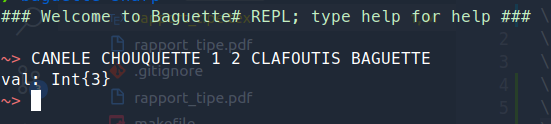
\includegraphics[width=0.6\textwidth]{img/add.png}
        \caption{Résultat dans le REPL de l'opération 1 + 2}
    \end{figure}
    
    La liste des mots clé de définitions est assez courte, il s'agit de \textit{IF,LABEL,JUMP} leur utilisation est expliquée \href{https://www.baguettesharp.fr/advanced.html#labels}{ici}
    à l'exception de ces mots clé, toutes les instructions doivent avoir leur paramètre entre parenthèse, les paramètres peuvent 
    être séparés par une virgule le \textit{lexer} ne les vois pas. Mais ils doivent être séparés par un espace au minimum (y compris avec une virgule)
    \begin{lstlisting}
        CANELE CHOUQUETTE 1 , 2 CLAFOUTIS BAGUETTE
    \end{lstlisting}
    est équivalent à 
    \begin{lstlisting}
        CANELE CHOUQUETTE 1 2 CLAFOUTIS BAGUETTE
    \end{lstlisting}
    Une explication complète de la syntaxe est disponible sur le \href{https://github.com/coco33920/ocaml-baguettesharp-interpreter/wiki/The-basics#syntax}{wiki-syntaxe}
    \subsection{Librairie Standard}
    Une liste complète des instructions est visible sur le \href{https://github.com/coco33920/ocaml-baguettesharp-interpreter/wiki}{wiki}
    et un tutoriel sur l'utilisation basique est disponible \href{https://www.baguettesharp.fr/basic.html}{ici}. La librairie 
    standard du langage implémente les usages suivants :
    \begin{itemize}
        \item Opération Mathématiques sur les entiers et flottant 
        \item Algèbre booléenne
        \item Lecture de l'entrée standard, écriture sur la sortie standard
        \item Manipulation de tableaux 
        \item Manipulation de chaînes de caractère
    \end{itemize}
    \bigskip


    Le langage est typé faiblement, et avec inférence de type, les types primitifs suivants sont implémentés
    \begin{itemize}
        \item Nombres entiers, flottants (NB: aucune distinction n'est faite entre les deux en général)
        \item Chaînes de caractères (NB: les caractères sont des chaînes de caractère de longueur 1)
        \item Booléans (\textit{CUPCAKE} est \textit{true} et \textit{POPCAKE} est \textit{false})
        \item Null (le \textit{unit} de OCaml)
    \end{itemize}
    \bigskip 

    Enfin le langage implémente les tableaux, à savoir qu'ils peuvent être \textit{non-homogène}
    donc vous pouvez faire un tableau contenant deux entiers, trois flottants et quatre chaînes de caractère
    cependant comme ce sont des tableaux ils sont de \textit{taille fixe} et ils héritent du caractère \textit{mutable}
    des tableaux de OCaml

    \section{Machine de Turing Binaire en \bs}
    Un moyen simple et ludique de montrer qu'un langage est Turing-complet est d'implémenter un émulateur d'une machine de Turing 
    universelle dans ce langage.\par 
    \bigskip 
    La machine de Turing et les programmes ont été adapté depuis \href{https://sandipanweb.wordpress.com/2020/08/08/simulating-a-turing-machine-with-python-and-executing-programs/}{ce} tutoriel sur une machine de turing universelle binaire 
    en python.
    \subsection{Spécification}
    Malheureusement on ne peut pas avoir une RAM infinie dans la réalité, voici la spécification de la machine qui est implémentée :
    \begin{itemize}
        \item Le ruban est de longueur 1000, initialisée avec 1000 "2" comme la machine est binaire le 2 est considéré comme étant le caractère 
        nul (une case vide)
        \item L'input est placée à partir de la place 500 dans le ruban, on place la tête au rang 500, au début de l'input.
        \item Les programmes sont une suite d'instruction de la forme STATE-READ-WRITE-TRANSLATION-NEWSTATE par exemple pour dire 
        que si on lit un 1 en étant dans l'état 0 alors on écrit un 2, on va à droite et on passe dans l'état 1 on écrira $0-1-2-r-1$
        \item On limite le tout à 100 states différents pour des raisons de performance, mais on peut augmenter en changeant la taille de la matrice.
        \item On appelle l'état de sortie "H", pour les déplacements 'r' déplace la tête d'une case vers la droite, 'l' d'une case 
        vers la gauche et '*' ne bouge pas la tête
    \end{itemize}
    \subsection{Initialisation}
    Ici est mise une image du code de l'initialisation.
    \begin{figure}[H]
        \begin{center}
        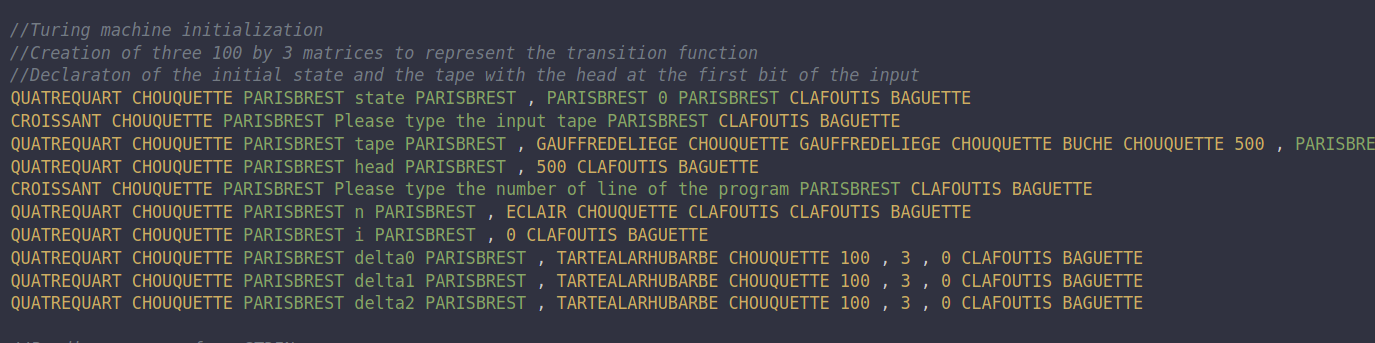
\includegraphics[width=\textwidth]{img/init.png}
        \caption{Initialisation de la machine}
        \end{center}
    \end{figure}
    En première ligne on initialise l'état initial de la machine à 0, puis on demande l'input tape (donc l'input) la ligne suivante n'est 
    pas affichée entièrement, elle initialise le ruban comme étant de longueur 500 puis on met l'input puis on remet 500 caractères vides (donc des 2)
    le plus important ici est les appels à l'instruction \textit{TARTEALARHUBARBE} qui construit une matrice de taille $n\times p$ (ici 100 par 3) initialisée 
    avec des 0. Ces trois matrices serviront à stocker le programme.
    Deux autres variable qui vont aider pour la boucle de lecture du programme sont initialisées il s'agit de $n$ le nombre de lignes du programme et de $i$ à 0. 
    \subsection{Lecture du programme}
    Pour lire le programme sur l'entrée standard, il nous faut émuler une boucle conditionnelle. Que le langage n'implémente pas nativement. 
    Pour cela nous aurons besoin des deux variables déclarés précédemment, $n$ et $i$. De l'instruction permettant de construire des labels $ICECREAM$,
    de l'instruction permettant de JUMP à un label $PAINVIENNOIS$ ainsi que d'un test conditionnel ici $SABLE$.\par 
    \bigskip 

    La boucle fait ceci dans l'ordre : 
    \begin{itemize}
        \item Lit l'entrée standard 
        \item Découpe la chaîne de caractère à tous les caractères "-" 
        \item Rempli les 3 matrices avec les programmes correspondant
        \item Incrémente $i$
        \item Vérifie si $i$ est supérieur ou égal à n
        \item Si $i\geq n$ alors il quitte le programme 
        \item Sinon il exécute un JUMP à lui-même
    \end{itemize}
    ces étapes rendent ceci une fois codées en \bs rendent 23 lignes de code (longues) disponible \href{https://github.com/coco33920/ocaml-baguettesharp-interpreter/blob/master/examples/turing.baguette#L3}{ici} 
    jusqu'à la ligne 23.\par 
    \bigskip 
    Ces étapes terminées le programme est lu et stocké dans les 3 matrices.

    \subsection{Étape}
    Il est ensuite nécessaire d'implémenter une \textit{étape} du programme. Là aussi, implémenté utilisant un label pour faire plus "propre" et pour séparer 
    les différentes fonctionnalités du programme -- les labels ne sont pas des \textit{fonctions} à proprement parler, et ensuite le \textit{scopes} des variables 
    est global, permettant d'émuler un peu le fonctionnement de véritables fonctions avec uniquement des labels. L'instruction la plus utilisée sera 
    \textit{TARTEAUXFRAISES} qui permet d'accéder à l'élément $n$ d'un tableau.\par 
    \bigskip 
    Une étape doit faire ceci : 
    \begin{itemize}
        \item Vérifier qu'on est bien dans un état différent de "H". La suite est dans le cas ou cette assertion est vraie
        \item Lire le ruban avec la tête de lecture pour obtenir l'état du ruban appelé $e$, l'état de la machine est $s$ 
        \item Récupérer ce que l'on doit écrire depuis la première matrice aux coordonnées $(s,e)$
        \item Récupérer dans quelle direction aller depuis la seconde matrice aux coordonnées $(s,e)$
        \item Récupérer le nouvel état de la machine depuis la troisième matrice aux coordonéées $(s,e)$
        \item Modifier le ruban en écrivant ce que l'on doit écrire 
        \item Mettre à jour l'état de la machine avec le nouvel état 
        \item Mettre à jour la position de la tête selon si on a lu $r$ $l$ ou * 
        \item Afficher le ruban (en enlevant les 2) et l'état de la machine
    \end{itemize} 
    L'implémentation en \bs de ce code est disponible une fois encore sur GitHub \href{https://github.com/coco33920/ocaml-baguettesharp-interpreter/blob/master/examples/turing.baguette#L26}{ici} jusqu'à la ligne 58
    Ce morceau de code fait uniquement \textit{une} étape. Il faut maintenant implémentée la boucle principale

    \subsection{Runtime de la machine}
    Maintenant qu'une étape de la machine a été implémentée il faut répéter les étapes tant que l'état de la machine est "H". 
    On verra dans les exemples comment le programme se comporte face à un programme qui ne s'arrête pas. Là encore nous avons affaire 
    à une boucle conditionnelle que l'on peut implémenter à l'aide d'un label et d'un test conditionnel\par \bigskip
    \begin{figure}[H]
        \center 
        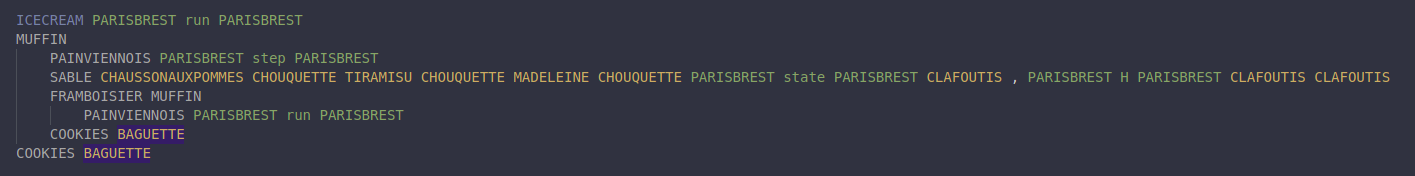
\includegraphics[width=\textwidth]{img/runtime.png}
        \caption{Runtime de la machine}
    \end{figure}
    Qui peut se traduire par "tant que l'état n'est pas 'H', on exécute step"
    Enfin, nous avons besoin d'ajouter un "JUMP "run"" juste après l'initialisation pour lancer le programme : 
    \begin{lstlisting}
        PAINVIENNOIS PARISBREST run PARISBREST
    \end{lstlisting}

    \section{Exemple de programmes}
    \subsection{left bit-shift}
    Le left-bitshift est une multiplication par 2 en binaire, c'est "bouger" tous les bits vers la gauche et ajouter un 0 à la fin.
    On peut faire ceci avec l'algorithme suivant 
    \begin{itemize}
        \item Si on est dans l'état 0 et qu'on lit un 0 on écrit un 0, on bouge à droite, et on reste dans l'état 0
        \item Si on est dans l'état 1 et qu'on lit un 1 on écrit un 1, on bouge à droite, et on reste dans l'état 0
        \item Si on est dans l'état 0 et qu'on lit un 2 on écrit un 0, on ne bouge pas et passe en état "H"
    \end{itemize}
    Sous forme d'automate (les transitions sont d'état de machine à état de machine, étiquetées par l'état du ruban lu)
    \begin{figure}[H]
        \center 
        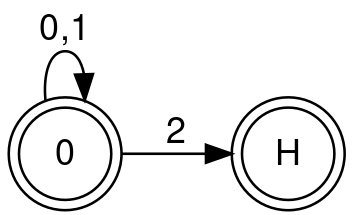
\includegraphics[width=0.5\textwidth]{img/automata1.png}
        \caption{Automate représentant le bitshift}
    \end{figure}
    Et sous forme de programme pour notre machine
    \begin{lstlisting}
        0-0-0-r-0
        0-1-1-r-0
        0-2-0-*-H
    \end{lstlisting}
    Dont l'exécution donne
    \begin{figure}[H]
        \center 
        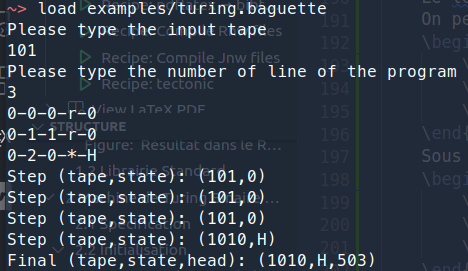
\includegraphics[width=0.5\textwidth]{img/bitshift.png}
        \caption{Exécution du left-bitshift}
    \end{figure}
    \subsection{Binary adder}
    Un additionneur binaire est bien plus complexe, le programme fait 17 lignes (et ne sera pas expliqué ici), rapidement 
    il se sert du deuxième chiffre comme d'un compteur pour additionner un par un au premier chiffre jusqu'à ce que le compteur atteigne 0.
    La représentation sous forme d'automate donne ceci
    \begin{figure}[H]
        \center 
        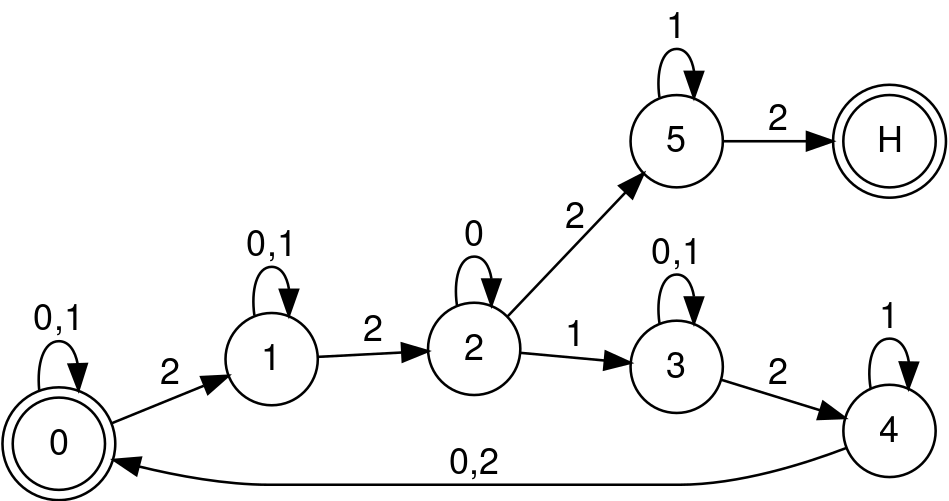
\includegraphics[width=0.5\textwidth]{img/automata2.png}
        \caption{Automate représentant l'addition binaire}
    \end{figure}
    Les 17 lignes du programme sont disponibles \href{https://github.com/coco33920/ocaml-baguettesharp-interpreter/blob/master/examples/turing_programs.txt#L5}{ici}
    l'exécution pour l'addition de 10 et 8 (en binaire 1010 et 1000) donne 10010 ce qui est bien 16+2 = 18.
    \begin{figure}[H]
        \center 
        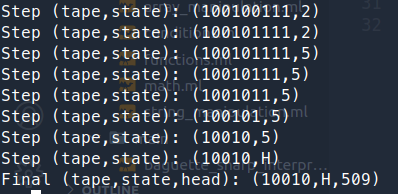
\includegraphics[]{img/adder.png}
        \caption{Dernières lignes de l'exécution de l'addition binaire}
    \end{figure}
    \subsection{Programme sans fin}
    Prenons un programme simple qui ne s'arrête pas :
    \begin{lstlisting}
        0-0-0-*-1
        1-0-0-*-0
    \end{lstlisting}
    Qui n'écris rien reste sur place et constamment passe de l'état 0 à 1 et vice versa.
    L'exécuter fait que l'interpréteur affiche pleins d'erreur jusqu'à s'arrêter et retourner sur le REPL.
    \begin{figure}[H]
        \center 
        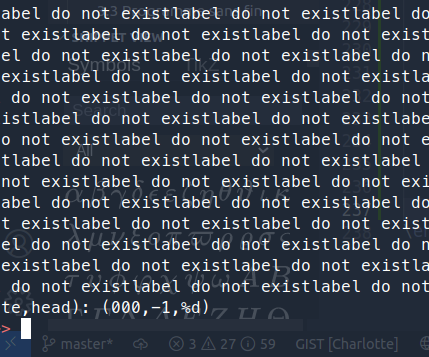
\includegraphics[width=0.5\textwidth]{img/error.png}
        \caption{Trace d'un programme sans fin}
    \end{figure}
\end{document}